\chapter{Código intermedio de CLANG/LLVM}

Clang es el \emph{frontend} de LLVM para la familia de los lenguajes de C. Clang consiste 
en un preprocesador C, un analizador léxico, un analizador sintáctico, un analizador 
semántico y un generador IR.
El Optimizador analiza la IR y la traduce a una forma más eficiente. \emph{opt} es la 
herramienta de optimización de LLVM.
El \emph{Backend} genera código máquina al mapear la IR al conjunto de instrucciones del 
hardware de destino. La herramienta backend de LLVM es llc. 
Genera código máquina a partir del IR de LLVM en tres fases: selección de instrucciones, 
asignación de registros y programación de la instrucción.

\begin{figure}[ht]
    \begingroup
        \centering
            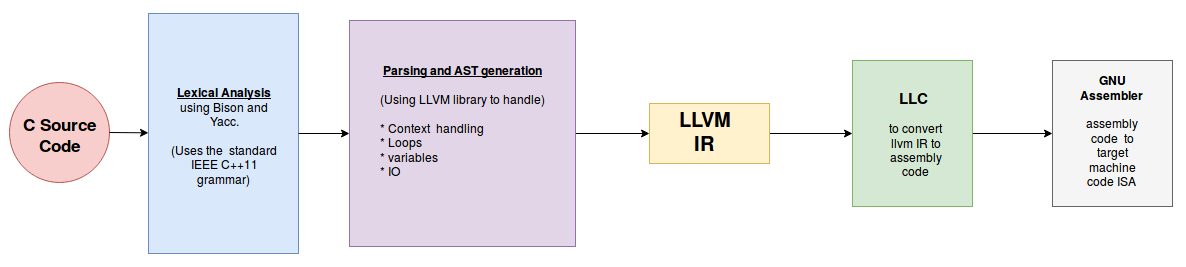
\includegraphics[width=1\textwidth,height=1\textheight,keepaspectratio]{clang process}
            \caption{Proceso de compilación de CLANG/LLVM.}
            \label{fig:clang process}
        \par
    \endgroup
\end{figure}

\section{Analizador léxico y sintáctico}

El analizador léxico lee la salida del preprocesador y realiza su tokenización.
El analizador sintáctico chequea si la gramática del lenguaje acepta la 
secuencia de \emph{tokens} generados por el analizador léxico y reporta errores de sintáxis.
El analizador sintáctico produce el \emph{error recovery}, si es posible.
La tokenización se organiza de la siguiente manera:
\begin{itemize}
    \item La definición del tipo de token en cuestión.
    \item El \emph{token}.
    \item \emph{Flag} que describe un adicional del \emph{token}.
    \item La ubicación del token en el código fuente.
\end{itemize}
Después de analizar la gramática de la secuencia de \emph{tokens}, 
emite un árbol abstracto sintáctico. Los nodos de un árbol abstracto sintáctico 
representan declaraciones, sentencias y tipos\cite{CLANGast}.

\begin{lstlisting}[label=comandoC, caption= Comando de compilación para obtener \emph{tokens} \cite{repositorio} para CLANG/LLVM., language=bash]
    $ clang -fsyntax-only -Xclang -dump-tokens codigo-ejemplo.c  2>&1 | tee tokens  \end{lstlisting}

\begin{lstlisting}[label=comandoC, caption= Comando de compilación para obtener ast \cite{repositorio} para CLANG/LLVM., language=bash]
    $ clang -fsyntax-only -Xclang -ast-dump codigo-ejemplo.c -fno-color-diagnostics > ast \end{lstlisting}

\section{Analizador semántico}
El analizador semántico recorre el árbol abstracto sintáctico, 
determinando si las sentencias del código tienen un significado válido. 
Esta fase comprueba los errores de tipo.

\section{LLVM IR}
El generador IR traduce el árbol abstracto sintáctico a código intermedio\cite{LLVMIR}. 

\begin{lstlisting}[label=comandoC, caption= Comando de compilación para obtener llvm-ir.ll \cite{repositorio} para CLANG/LLVM., language=bash]
    $ clang -S -emit-llvm codigo-ejemplo.c -o llvm-ir.ll \end{lstlisting}

En esta fase tambien trabaja el optimizador que mejora la eficiencia del código basándose 
en su comprensión del comportamiento en tiempo de ejecución del programa. 

\begin{lstlisting}[label=comandoC, caption= Comando de compilación para obtener llvm-ir-optimizedd.ll \cite{repositorio} para CLANG/LLVM., language=bash]
    $ opt -O2 -S llvm-ir.ll -o llvm-ir-optimized.ll \end{lstlisting}

\section{Selección de instrucciones} 

La selección de instrucciones es el mapeo de instrucciones IR al conjunto 
de instrucciones de la máquina de destino. Este paso utiliza un espacio de 
nombres infinito de registros virtuales.

\section{Asignación de registros} 

La asignación de registros es el mapeo de registros virtuales a registros 
reales en la arquitectura de destino.

\section{Programación de la instrucción}

La programación de la instrucción es la reordenación de operaciones para 
reflejar las restricciones de funcionamiento de la máquina de destino\cite{LLVMdocs}.

\begin{lstlisting}[label=comandoC, caption= Comando de compilación para obtener machineinstrs \cite{repositorio} para CLANG/LLVM., language=bash]
    $ llc llvm-ir.ll -print-machineinstrs 2>&1 tee machineinstrs \end{lstlisting}

\section{\emph{Assembler}}
Por último, es posible obtener la salida en lenguaje \emph{assembler} del código fuente.

\begin{lstlisting}[label=comandoC, caption= Comando de compilación para obtener assembly.s \cite{repositorio} para CLANG/LLVM., language=bash]
    $ llc llvm-ir.ll -o assembly.s \end{lstlisting}

